\begin{frame}[c]{Homogeneous example}
	\begin{figure}
		\centering
		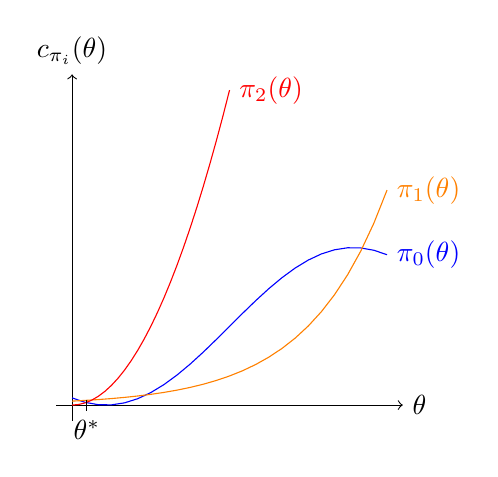
\begin{tikzpicture}
			%	\draw[very thin,color=gray] (-0.1,-1.1) grid (3.9,3.9);
			\draw[->] (-0.2,0) -- (4.2,0) node[right] {$\theta$};
			\draw[->] (0,-0.2) -- (0,4.2) node[above] {$c_{\pi_i}(\theta)$};
			\draw[color=blue,domain=0:4]   plot (\x,{sin((\x-2) r) + 1})   node[right] {$\pi_0(\theta)$};
			\draw[color=orange,domain=0:4] plot (\x,{0.05*exp(\x)}) node[right] {$\pi_1(\theta)$};
			\draw[color=red,domain=0:2] plot (\x,{\x*\x}) node[right] {$\pi_2(\theta)$};
			
			\only<2>{
				\foreach \x/\xtext in {0.1875/\theta^*}
					\draw[shift={(\x,0)}] (0pt,2pt) -- (0pt,-2pt) node[below] {$\xtext$};
			}
		\end{tikzpicture}
	\end{figure}
\end{frame}

\begin{frame}[c]{Heterogeneous example}
	\begin{figure}
		\centering
			\begin{tikzpicture}
			%	\draw[very thin,color=gray] (-0.1,-1.1) grid (3.9,3.9);
			\draw[->] (-0.2,0) -- (4.2,0) node[right] {$\theta$};
			\draw[->] (0,-0.2) -- (0,4.2) node[above] {$c_{\pi_i}(\theta)$};
			\draw[color=blue,domain=3:7]   plot (\x-3,{sin((\x-2) r) + 1.275})   node[right] {$\pi_0(\theta)$};
			\draw[color=orange,domain=0:4] plot (\x,{0.05*exp(\x)}) node[right] {$\pi_1(\theta)$};
			\draw[color=red,domain=-2:2] plot (\x+2,{\x*\x}) node[right] {$\pi_2(\theta)$};
			
			\only<2->{
				 \foreach \x/\xtext in {0/\theta_{\pi_1}^*, 2/\theta_{\pi_0}^*, 3.725/\theta_{\pi_2}^*}
					\draw[shift={(\x,0)}] (0pt,2pt) -- (0pt,-2pt) node[below] {$\xtext$};
			}
			\only<3->{
				 \foreach \y/\ytext in {.75/c_{\theta_{SB}}}
					\draw[shift={(0,\y)}] (2pt,0pt) -- (-2pt,0pt) node[left] {$\ytext$};
				 \foreach \x/\xtext in {2.725/\theta_{SB}}
					\draw[shift={(\x,0)}] (0pt,2pt) -- (0pt,-2pt) node[below] {$\xtext$};
				 \draw[densely dotted,color=gray] (0,0.75) -- (2.725,.75);
				 \draw[densely dotted,color=gray] (2.725,0) -- (2.725,.75);
			}
			\only<4->{
			%	\draw[dashed,color=gray] (0,0.1275) -- (3.725,0.1275);
				\foreach \y/\ytext in {0.1275/c_{oracle}}
				\draw[shift={(0,\y)}] (2pt,0pt) -- (-2pt,0pt) node[left] {$\ytext$};
			}
			\end{tikzpicture}
	\end{figure}
\end{frame}

\begin{frame}[c]{Hydra: Iteration 0}
	\begin{figure}
		\centering
		\begin{tikzpicture}
		
			\only<1>{
				%	\draw[very thin,color=gray] (-0.1,-1.1) grid (3.9,3.9);
				\draw[->] (-0.2,0) -- (4.2,0) node[right] {$\theta$};
				\draw[->] (0,-0.2) -- (0,4.2) node[above] {$c_{\pi_i}(\theta)$};
				\draw[color=blue,domain=3:7]   plot (\x-3,{sin((\x-2) r) + 1.275})   node[right] {$\pi_0(\theta)$};
				\draw[color=orange,domain=0:4] plot (\x,{0.05*exp(\x)}) node[right] {$\pi_1(\theta)$};
				\draw[color=red,domain=-2:2] plot (\x+2,{\x*\x}) node[right] {$\pi_2(\theta)$};
				
%				\foreach \y/\ytext in {.75/c_{\theta_{0}}}
%				\draw[shift={(0,\y)}] (2pt,0pt) -- (-2pt,0pt) node[left] {$\ytext$};
				\foreach \x/\xtext in {2.725/\theta_{0}}
				\draw[shift={(\x,0)}] (0pt,2pt) -- (0pt,-2pt) node[below] {$\xtext$};
%				\draw[densely dotted,color=gray] (0,0.75) -- (2.725,.75);
				\draw[densely dotted,color=gray] (2.725,0) -- (2.725,4);
			}
			\only<2>{
				%Update metric
				%	\draw[very thin,color=gray] (-0.1,-1.1) grid (3.9,3.9);
				\draw[->] (-0.2,0) -- (4.2,0) node[right] {$\theta$};
				\draw[->] (0,-0.2) -- (0,4.2) node[above] {$c_{\pi_i}^{'}(\theta)$};
				
				\draw[color=orange,domain=0:2.725] plot (\x,{0.05*exp(\x)});
				\draw[color=orange,domain=2.725:4] plot (\x,.75) node[right] {$\pi_1(\theta)$};
				
				\draw[color=red,domain=-.725:.725] plot (\x+2,{\x*\x});
				\draw[color=red,domain=-2:-.725] plot (\x+2,0.525625);
				\draw[color=red,domain=.725:2] plot (\x+2,0.525625) node[right] {$\pi_2(\theta)$};
				
				\draw[color=blue,domain=5.725:7]   plot (\x-3,{sin((\x-2) r) + 1.275})   node[right] {$\pi_0(\theta)$};
				\draw[color=blue,domain=3:5.725]   plot (\x-3,.75);
				
				\foreach \y/\ytext in {.75/c^{'}_{\pi_{\left\{0, 1\right\}}}(\mathcal{P})}
				\draw[shift={(0,\y)}] (2pt,0pt) -- (-2pt,0pt) node[left,yshift=0.15cm] {$\ytext$};
				\foreach \y/\ytext in {0.525625/c^{'}_{\pi_{2}}(\mathcal{P})}
				\draw[shift={(0,\y)}] (2pt,0pt) -- (-2pt,0pt) node[left,yshift=-0.15cm] {$\ytext$};
				
				\foreach \x/\xtext in {2.725/\theta_{0}}
				\draw[shift={(\x,0)}] (0pt,2pt) -- (0pt,-2pt) node[below] {$\xtext$};
				
%				\draw[densely dotted,color=gray] (0,0.75) -- (2.725,.75);
				\draw[densely dotted,color=gray] (2.725,0) -- (2.725,.75);
			}
		\end{tikzpicture}
		\caption{
			\only<1>{Search initial well performing configuration. Add $\theta_{0}$ to $\mathcal{P}$}
			\only<2>{Update metric}
		}
	\end{figure}
\end{frame}



\begin{frame}[c]{Hydra: Iteration 1}
\begin{figure}
	\centering
	\begin{tikzpicture}
	\only<1>{
		%Update metric
		%	\draw[very thin,color=gray] (-0.1,-1.1) grid (3.9,3.9);
		\draw[->] (-0.2,0) -- (4.2,0) node[right] {$\theta$};
		\draw[->] (0,-0.2) -- (0,4.2) node[above] {$c_{\pi_i}^{'}(\theta)$};
		
		\draw[color=orange,domain=0:2.725] plot (\x,{0.05*exp(\x)});
		\draw[color=orange,domain=2.725:4] plot (\x,.75) node[right] {$\pi_1(\theta)$};
		
		\draw[color=red,domain=-.725:.725] plot (\x+2,{\x*\x});
		\draw[color=red,domain=-2:-.725] plot (\x+2,0.525625);
		\draw[color=red,domain=.725:2] plot (\x+2,0.525625) node[right] {$\pi_2(\theta)$};
		
		\draw[color=blue,domain=5.725:7]   plot (\x-3,{sin((\x-2) r) + 1.275})   node[right] {$\pi_0(\theta)$};
		\draw[color=blue,domain=3:5.725]   plot (\x-3,.75);
		
		\foreach \y/\ytext in {.75/c^{'}_{\pi_{\left\{0, 1\right\}}}(\mathcal{P})}
		\draw[shift={(0,\y)}] (2pt,0pt) -- (-2pt,0pt) node[left,yshift=0.15cm] {$\ytext$};
		\foreach \y/\ytext in {0.525625/c^{'}_{\pi_{2}}(\mathcal{P})}
		\draw[shift={(0,\y)}] (2pt,0pt) -- (-2pt,0pt) node[left,yshift=-0.15cm] {$\ytext$};
		
		\foreach \x/\xtext in {2.725/\theta_{0}, 3.725/\theta_{1}}
		\draw[shift={(\x,0)}] (0pt,2pt) -- (0pt,-2pt) node[below] {$\xtext$};
		
%		\draw[densely dotted,color=gray] (0,0.75) -- (2.725,.75);
		\draw[densely dotted,color=gray] (2.725,0) -- (2.725,.75);
		\draw[densely dotted,color=gray] (3.725,0) -- (3.725,4);
	}

	\only<2>{
		%Update metric
		%	\draw[very thin,color=gray] (-0.1,-1.1) grid (3.9,3.9);
		\draw[->] (-0.2,0) -- (4.2,0) node[right] {$\theta$};
		\draw[->] (0,-0.2) -- (0,4.2) node[above] {$c_{\pi_i}^{''}(\theta)$};
		
		\draw[color=orange,domain=0:2.725] plot (\x,{0.05*exp(\x)});
		\draw[color=orange,domain=2.725:4] plot (\x,.75) node[right] {$\pi_1(\theta)$};
		
		\draw[color=red,domain=-.725:.725] plot (\x+2,{\x*\x});
		\draw[color=red,domain=-2:-.725] plot (\x+2,0.525625);
		\draw[color=red,domain=.725:2] plot (\x+2,0.525625) node[right] {$\pi_2(\theta)$};
		
		\draw[color=blue,domain=0:4]   plot (\x,.25)   node[right] {$\pi_0(\theta)$};
%		\draw[color=blue,domain=3:5.725]   plot (\x-3,.75);
		
		\foreach \y/\ytext in {.75/c_{\pi_{1}}^{''}(\mathcal{P})}
		\draw[shift={(0,\y)}] (2pt,0pt) -- (-2pt,0pt) node[left,yshift=0.1cm] {$\ytext$};
		\foreach \y/\ytext in {0.525625/c_{\pi_{2}}^{''}(\mathcal{P})}
		\draw[shift={(0,\y)}] (2pt,0pt) -- (-2pt,0pt) node[left,yshift=-0.0cm] {$\ytext$};
		\foreach \y/\ytext in {0.25/c_{\pi_{0}}^{''}(\mathcal{P})}
		\draw[shift={(0,\y)}] (2pt,0pt) -- (-2pt,0pt) node[left,yshift=-0.0cm] {$\ytext$};
		
		\foreach \x/\xtext in {2.725/\theta_{0}, 3.725/\theta_{1}}
		\draw[shift={(\x,0)}] (0pt,2pt) -- (0pt,-2pt) node[below] {$\xtext$};
		
				\draw[densely dotted,color=gray] (0,0.75) -- (2.725,.75);
		\draw[densely dotted,color=gray] (2.725,0) -- (2.725,.75);
		\draw[densely dotted,color=gray] (3.725,0) -- (3.725,.25);
	}
	\end{tikzpicture}
	\caption{
		\only<1>{Search well performing configuration complementary to $\mathcal{P}$.\\Add $\theta_{1}$ to $\mathcal{P}$.}
		\only<2>{Update metric}
	}
\end{figure}
\end{frame}





\begin{frame}[c]{Hydra: Iteration 2}
\begin{figure}
	\centering
	\begin{tikzpicture}
	
	\only<1>{
		%Update metric
		%	\draw[very thin,color=gray] (-0.1,-1.1) grid (3.9,3.9);
		\draw[->] (-0.2,0) -- (4.2,0) node[right] {$\theta$};
		\draw[->] (0,-0.2) -- (0,4.2) node[above] {$c_{\pi_i}^{''}(\theta)$};
		
		\draw[color=orange,domain=0:2.725] plot (\x,{0.05*exp(\x)});
		\draw[color=orange,domain=2.725:4] plot (\x,.75) node[right] {$\pi_1(\theta)$};
		
		\draw[color=red,domain=-.725:.725] plot (\x+2,{\x*\x});
		\draw[color=red,domain=-2:-.725] plot (\x+2,0.525625);
		\draw[color=red,domain=.725:2] plot (\x+2,0.525625) node[right] {$\pi_2(\theta)$};
		
		\draw[color=blue,domain=0:4]   plot (\x,.25)   node[right] {$\pi_0(\theta)$};
		%		\draw[color=blue,domain=3:5.725]   plot (\x-3,.75);
		
		\foreach \y/\ytext in {.75/c_{\pi_{1}}^{''}(\mathcal{P})}
		\draw[shift={(0,\y)}] (2pt,0pt) -- (-2pt,0pt) node[left,yshift=0.1cm] {$\ytext$};
		\foreach \y/\ytext in {0.525625/c_{\pi_{2}}^{''}(\mathcal{P})}
		\draw[shift={(0,\y)}] (2pt,0pt) -- (-2pt,0pt) node[left,yshift=-0.0cm] {$\ytext$};
		\foreach \y/\ytext in {0.25/c_{\pi_{0}}^{''}(\mathcal{P})}
		\draw[shift={(0,\y)}] (2pt,0pt) -- (-2pt,0pt) node[left,yshift=-0.0cm] {$\ytext$};
		
		\foreach \x/\xtext in {2.725/\theta_{0}, 3.725/\theta_{1}, 2/\theta_{2}}
		\draw[shift={(\x,0)}] (0pt,2pt) -- (0pt,-2pt) node[below] {$\xtext$};
		
		\draw[densely dotted,color=gray] (0,0.75) -- (2.725,.75);
		\draw[densely dotted,color=gray] (2.725,0) -- (2.725,.75);
		\draw[densely dotted,color=gray] (3.725,0) -- (3.725,.25);
		\draw[densely dotted,color=gray] (2,0) -- (2,4);
	}

	\only<2>{
		%Update metric
		%	\draw[very thin,color=gray] (-0.1,-1.1) grid (3.9,3.9);
		\draw[->] (-0.2,0) -- (4.2,0) node[right] {$\theta$};
		\draw[->] (0,-0.2) -- (0,4.2) node[above] {$c_{\pi_i}^{'''}(\theta)$};
		
		\draw[color=orange,domain=0:2] plot (\x,{0.05*exp(\x)});
		\draw[color=orange,domain=2:4] plot (\x,.369) node[right,yshift=.25cm] {$\pi_1(\theta)$};
		
		\draw[color=red,domain=0:4] plot (\x,0) node[right,xshift=.5cm] {$\pi_2(\theta)$};
		
		\draw[color=blue,domain=0:4]   plot (\x,.25)   node[right] {$\pi_0(\theta)$};
		%		\draw[color=blue,domain=3:5.725]   plot (\x-3,.75);
		
		\foreach \y/\ytext in {.369/c_{\pi_{1}}^{'''}(\mathcal{P})}
		\draw[shift={(0,\y)}] (2pt,0pt) -- (-2pt,0pt) node[left,yshift=0.25cm, xshift=1.3cm] {$\ytext$};
		\foreach \y/\ytext in {0/c_{\pi_{2}}^{'''}(\mathcal{P})}
		\draw[shift={(0,\y)}] (2pt,0pt) -- (-2pt,0pt) node[left,yshift=-0.25cm, xshift=1.3cm] {$\ytext$};
		\foreach \y/\ytext in {0.25/c_{\pi_{0}}^{'''}(\mathcal{P})}
		\draw[shift={(0,\y)}] (2pt,0pt) -- (-2pt,0pt) node[left,yshift=-0.0cm] {$\ytext$};
		
		\foreach \x/\xtext in {2.725/\theta_{0}, 3.725/\theta_{1}, 2/\theta_{2}}
		\draw[shift={(\x,0)}] (0pt,2pt) -- (0pt,-2pt) node[below] {$\xtext$};
		
		\draw[densely dotted,color=gray] (0,.369) -- (2,.369);
		\draw[densely dotted,color=gray] (2.725,0) -- (2.725,.369);
		\draw[densely dotted,color=gray] (3.725,0) -- (3.725,.25);
		\draw[densely dotted,color=gray] (2,0) -- (2,.369);
	}
	\end{tikzpicture}
	\caption{
		\only<1>{Search well performing configuration complementary to $\mathcal{P}$.\\Add $\theta_{2}$ to $\mathcal{P}$.}
		\only<2>{Update metric}
	}
\end{figure}
\end{frame}